\documentclass[11pt]{article}
\usepackage[utf8]{inputenc}
\usepackage{polski}
\usepackage{graphicx}
\usepackage{array}
\usepackage{paralist}
\usepackage{verbatim}
\usepackage{fancyvrb}
\usepackage{subfig}
\usepackage{amsmath}
\usepackage{float}
\usepackage{amsthm}
\usepackage{amssymb}
\usepackage{pdfpages}
\usepackage{amsfonts}
\usepackage{tikz}
\usepackage{wasysym}
\usepackage[linguistics]{forest}
\usetikzlibrary{shapes,backgrounds}
\usepackage[margin=1in]{geometry}
% \setlength\parindent{0pt}
% \theoremstyle{definition}
% \newtheorem{zadanie}{Zadanie}
% \numberwithin{zadanie}{subsection}
% \renewcommand*{\proofname}{Rozwiązanie}


\title{Systemy operacyjne 1}
\author{Igor Nowicki}
\begin{document}
\maketitle
\tableofcontents

\section{Wprowadzenie do wielodostępnych systemów operacyjnych}

\begin{figure}[H]
    \centering
    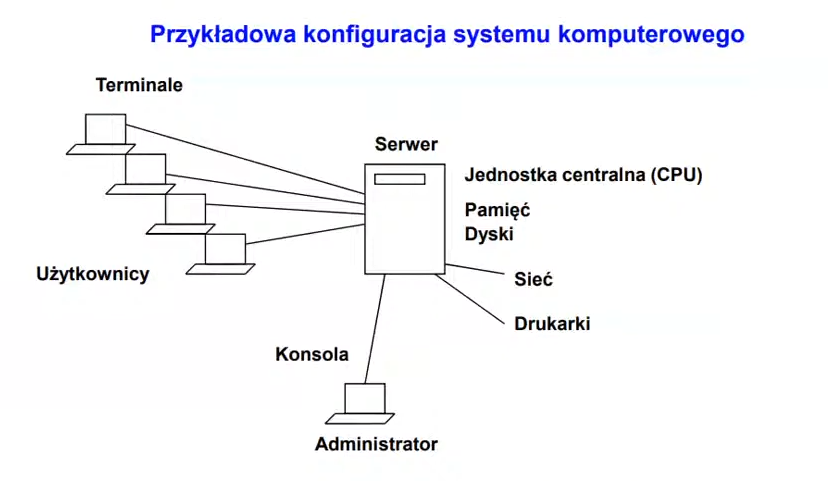
\includegraphics[width=0.5\linewidth]{./img/so1-01.png}
\end{figure}

System operacyjny: program zarządzający pracą komputera

Zadania użytkownika wykonywane są jako procesy obsługiwane przez system
operacyjny. System przydziela procesom zasoby komputera: dostęp do jednostki
centralnej, pamięć, dyski, i inne.

Niezbędny administrator - osoba odpowiedzialna za sprawne działanie i bezpieczeństwo
systemu. Również opiekun użytkowników, zakłada konta użytkowników, służy pomocą i
radą.

\begin{figure}[H]
    \centering
    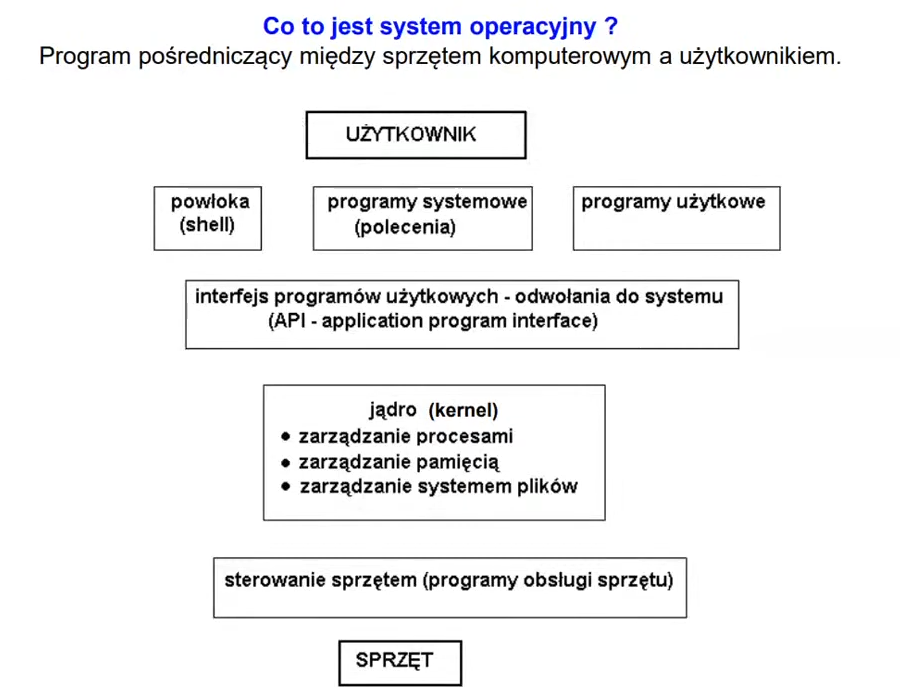
\includegraphics[width=0.5\linewidth]{./img/so1-02.png}
\end{figure}

Ani użytkownik, ani proces wywoływany bezpośrednio przez użytkownika nie ma bezpośredniego dostępu do sprzętu. Jeśli użytkownik chce skorzystać ze sprzętu, musi wywołać odwołanie poprzez API.

\subsection{Podstawowe cechy systemu operacyjnego}

\subsection{Części składowe systemu operacyjnego.}

\subsection{Struktura systemu operacyjnego}

\subsection{Usługi systemu operacyjnego.}



\subsection{Co to jest system operacyjny?}
Program pośredniczący między sprzętem komputerowym a użytkownikiem.

(kernel)

Krótka historia systemu operacyjnego UNIX

Dlaczego UNIX stał się popularny?
\begin{itemize}
    \item mały, elastyczny, tani, dostępny na komputerach od micro do super komputerów
    \item właściwości zazwyczaj dostępne tylko w dużych systemach operacyjnych:
    \item architektura wieloprocesowa, inicjowanie asynchronicznych procesów
    \item hierarchiczny system plików
\end{itemize}

\subsection{Cele standaryzacji}
Budowa systemów tzw. "otwartych", charakteryzujących się:
\begin{itemize}
    \item przenośnością aplikacji (portability),
    \item możliwością współpracy oprogramowania działającego na różnych maszynach (interoperability),
    \item skalowalnością (scalability), t.j. możliwością rozbudowy sprzętowej i rozbudowy aplikacji bez
          konieczności zmian systemu.
\end{itemize}
Istota standardu: określenie interfejsu, a nie implementacji.

\subsection{Niektóre standardy i instytucje standaryzujące}

SVID - standard firmy AT\&T - pierwsza próba standardu interfejsu systemu operacyjnego.

POSIX - standard sponsorowany przez Instytut IEEE (Institute of Electrical and Electronics
Engineering). Prace nad tym standardem obejmują: interfejs systemu, programy shell, metody
testowania zgodności danego systemu ze standardem, pracę w sieci, zagadnienia ochrony i inne.

OSF (Open System Foundation) stowarzyszenie wiodących firm: HP, IBM, DEC i innych,
zajmujące się promocją systemów otwartych. Opracowany został standard OSF/Motif.
Aktualne prace obejmują między innymi: Distributed Computing Environment - przetwarzanie w
środowisku rozproszonym, Distributed Management Environment - centralne zarządzanie sieciami
heterogenicznymi.

ISO - International Standard Organization - koordynuje tworzenie i stosowanie standardów w skali
międzynarodowej. Wprowadziła siedmiowarstwowy model odniesienia OSI (Open System
Interconnection) dotyczący pracy w sieciach komputerowych.

\subsection{Cechy systemu UNIX}

\begin{itemize}
    \item System wielodostępny (ang. multiuser): wielu użytkowników pracujących z jednym komputerem, wrażenie samodzielnej pracy
    \item Praca interakcyjna (interactive):
          użytkownik wprowadza polecenie z terminala, UNIX wykonuje polecenie, wyświetla wyniki i czeka na nowe polecenie każdy
    \item System wielozadaniowy (multitasking): użytkownik może uruchomić jednocześnie wiele programów
    \item Zapewnia bezpieczeństwo (security, privacy): identyfikacja użytkowników, ochrona dostępu do plików i katalogów, ochrona procesów
    \item Niezależny od urządzeń system we/wy (device independent I/O): każde urządzenie reprezentowane jest przez plik specjalny systemu
    \item Komunikacja między procesami (ang. interprocess communication): aplikacje mogą wzajemnie się ze sobą komunikować
    \item System sieciowy (networking): wbudowane jest oprogramowanie umożliwiające pracę w sieci
    \item Polecenie/Program użytkowy (commands/utilities): polecenie jest programem użytkowym, można samemu je napisać
    \item Interpretator poleceń (shell): jest wiele programów shell'a, można go zmienić
\end{itemize}


\subsection{Struktura systemu operacyjnego}

Podsystemy wykonujące zadania:

\begin{itemize}
    \item Zarządzanie procesami: tworzenie, usuwanie, zawieszanie, odwieszanie procesów, mechanizmy
          synchronizacji procesów, komunikacja między procesami.

    \item Zarządzanie pamięcią: zarządzanie pamięcią główną, obszarem wymiany (swap), pojęcie
          pamięci wirtualnej.

    \item Zarządzanie przestrzenią dyskową: zarządzanie wolną przestrzenią dysków, procesami,
          zapisywania informacji na dysku, szeregowanie zadań zapisu i odczytu.

    \item Zarządzanie operacjami we/wy: obejmuje podsystem buforowania,

    \item interfejs: urządzenia -sterowniki, sterowniki urządzeń.

    \item Zarządzanie plikami: tworzenie, usuwanie plików i katalogów,
          elementarne operacje z plikami i katalogami.

    \item Podsystem ochrony: ochrona procesów przed działaniem innych procesów, mechanizmy
          zapewniające, że pliki, segmenty pamięci, CPU, inne zasoby są udostępnione tylko tym
          procesom, które mają autoryzację systemu operacyjnego. Ogólnie: mechanizmy kontroli dostępu
          programów, procesów, użytkowników do zasobów systemu komputerowego.

    \item Praca sieciowa: usługi umożliwiające komunikację w sieci,
          pojęcie systemów rozproszonych.
\end{itemize}

\subsection{Usługi systemu operacyjnego}
\begin{itemize}
    \item Wykonywanie programów
    \item Operacje we/wy
    \item Operacje obsługi systemu plików
    \item Komunikacja między procesami
    \item Detekcja błędów
    \item Przydział zasobów
    \item Rozliczanie użytkowników (accounting)
    \item Ochrona
    \item Funkcje systemowe (system calls):
    \item interfejs między procesami i systemem operacyjnym
\end{itemize}

\begin{figure}[H]
    \centering
    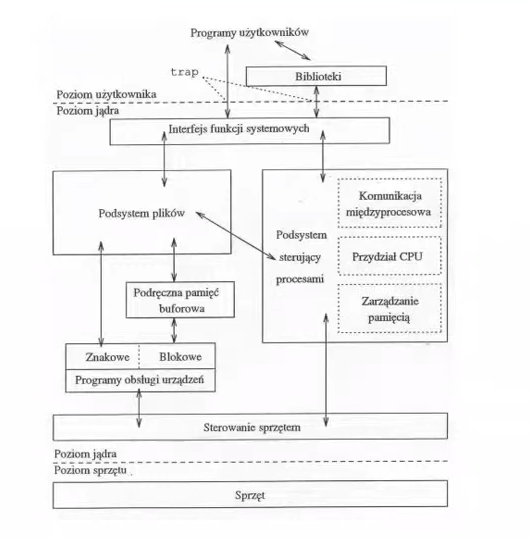
\includegraphics[width=0.5\linewidth]{./img/so1-03.png}
\end{figure}

Przykłady funkcji systemowych (system calls):

Podsystem plików:
open, read, write, stat

chown, chmod

Podsystem sterowania procesami:

fork, exec, exit, wait, signal

\subsection{Pytania}

\begin{enumerate}
    \item Co to jest system operacyjny? Jakie funkcje spełnia?

          System operacyjny to program pośredniczący między sprzętem
          komputerowym a użytkownikiem. Zadania użytkownika
          wykonywane są jako procesy obsługiwane przez system
          operacyjny. System przydziela procesom zasoby komputera:
          dostęp do jednostki centralnej, pamięć, dyski, i inne.

    \item Co to są funkcje systemowe?


          Funkcje systemowe (system call) – stanowią interfejs między
          wykonywanym programem a (posiadającym zwykle wyższe
          uprawnienia) jądrem systemu operacyjnego. Funkcje systemowe
          wywoływane są przez specjalny mechanizm, wspierany przez dany
          procesor, na przykład z użyciem wyznaczonego przerwania lub
          instrukcji skoku dalekiego.
          Podsystem plików:
          Przyklady:
          \begin{itemize}
              \item open, read, write, stat (stan)
              \item Chown (zmiana właściciela)
              \item chmod
          \end{itemize}

          Sterowanie procesami:
          \begin{itemize}
              \item Fork (utworzenie nowego procesu, nowy proces-klon istniejącego procesu),
              \item Exec (umozliwia działanie nowego procesu tak jak chcemy),
              \item exit
              \item Wait,
              \item signal (możliwość wysylania sygnalu do danego procesu)
          \end{itemize}
    \item Co jest przedmiotem standaryzacji systemów otwartych?

          Ujednolicenie systemu, języka maszynowego, zasad działania,
          nazywania, odszukiwania plików, aby dla każdego użytkownika
          była taka sama.
          stworzenie kryteriów schematu ich wykonywania.
          eliminowanie błędów przez co wzrasta efektywność działania
          systemu.
          Rozne wersje systemow uzyte w jednolitym systemie
          komputerowym.
\end{enumerate}

\section{Systemy plików}

\subsection{Pliki i systemy plików w systemie operacyjnym}

Pliki to jednostki logiczne przechowywanej informacji, niezależne od właściwości fizycznych
urządzeń pamięciowych. Zwykłe w plikach przechowywane są programy lub dane (tekst, liczby,
grafika, itp.).

System plików - zbiór typów danych, struktur danych oraz funkcji systemowych (ang. system
calls) używanych przez system operacyjny w celu przechowywania informacji w urządzeniach
pamięci masowej (głównie na dyskach).

W systemach wielodostępnych systemy plików mają strukturę katalogową (hierarchiczną).
Pliki identyfikuje się za pomocą nazw. W systemie UNIX, w zależności od implementacji, pliki
mogą mieć krótkie nazwy, do 14 znaków, lub długie nazwy, do 255 znaków.

Zestaw znaków dopuszczalnych obejmuje:

małe lub duże litery, cyfry, znaki specjalne takie jak \verb{,,+, - , _' ."}

Przykład

Dopuszczalne nazwy plików: \verb{.profile .xyz.abcd abc AbC 123..456..78 -a}

UWAGA: Tej ostatniej nazwy lepiej jednak nie używać.

UWAGA: W systemie UNIX pliki mogą być identyfikowane za pomocą wielu różnych nazw (dowiązań).

\subsection{Podstawowe typy plików}

Podstawowe typy plików: pliki zwykłe, pliki specjalne (urządzeń), katalogi, potoki nazwane, gniazda.
\begin{itemize}
    \item pliki zwykłe,

          W plikach zwykłych przechowujemy programy, dane, teksty, grafikę, itp.
          W systemie UNIX pliki zwykłe nie mają ustalonego formatu. Plik zwykły jest po prostu ciągiem bajtów o danej
          długości. Oczywiście aplikacje mogą tworzyć pliki o ściśle ustalonym formacie,
          na przykład plik assembler generuje plik, w którym wyróżniamy: nagłówek, kod wykonywalny, inicjalizowane dane.

    \item pliki specjalne,

          Pliki specjalne, nazywane również plikami urządzeń zapewniają łączność z urządzeniami,
          na przykład z dyskami, terminalami, napędami taśmy, itp. W plikach specjalnych nie
          przechowuje się żadnych danych. Pliki te charakteryzują sposób działania urządzenia,
          wskazują miejsce podłączenia urządzeń do systemu oraz zapewniają dostęp do
          programów obsługi urządzeń („drajwerów”).

    \item katalogi,

          Katalogi służą do powiązania nazw plików z danymi znajdującymi się na dysku. W każdym
          katalogu może znajdować się pewna liczba plików i innych katalogów (podkatalogów).
          Katalog jest przechowywany jak plik zwykły i (w uproszczeniu) ma postać tabeli o dwóch
          kolumnach. Każdy wiersz tej tabeli zawiera nazwę pliku znajdującego się w katalogu (lub
          podkatalogu) oraz pewien numer, pozwalający na odszukanie atrybutów pliku i danych,
          które się w nim znajdują.

    \item dowiązania symboliczne - operacja nadania dodatkowej nazwy istniejącemu plikowi,

          Dowiązania zwykłe mogą być tworzone w obrębie tego samego systemu plików.
          Dowiązań symbolicznych używa się ponad granicami systemów plików oraz w
          odniesieniu do katalogów. Przechowywane są w nich ścieżki dostępu do plików lub
          katalogów, na które dowiązania te wskazują.

    \item potoki nazwane FIFO (ang. named pipe),

          Potoki nazwane (FIFO) wykorzystywane są do komunikacji między procesami.
          Do tworzenia tych potoków wykorzystywane są odpowiednie procedury biblioteczne.
          Procesy mogą otwierać potoki nazwane do odczytu i zapisu, tak jak otwierają pliki zwykłe.
          Gniazda wprowadzone zostały w systemie BSD UNIX. Są wykorzystywane również do
          komunikacji między procesami. Wykorzystują jednak inne mechanizmy niż potoki
          nazwane.

    \item gniazda (ang. UNIX--domain sockets).
\end{itemize}

\begin{figure}[H]
    \centering
    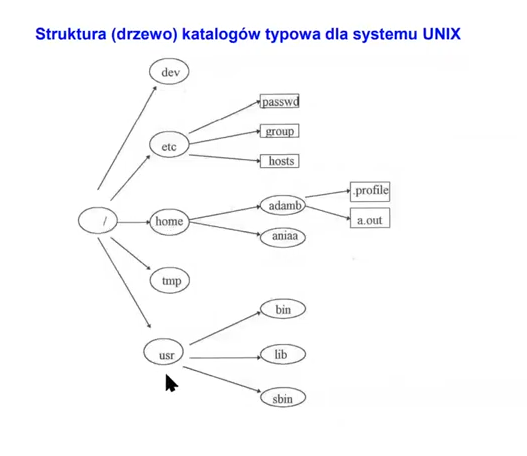
\includegraphics[width=0.5\linewidth]{./img/so1-04.png}
\end{figure}




\subsection{Ścieżka dostępu}

Struktura systemu plików w systemie UNIX.

Jeden z katalogów zawsze służy użytkownikowi pracującemu w systemie UNIX jako katalog bieżący.

Położenie pliku lub katalogu w drzewie katalogów określa ścieżka dostępu do pliku lub katalogu.
Bezwzględna ścieżka dostępu określa położenie pliku lub katalogu względem katalogu głównego

(ang. root directory) 
\verb /
, na przykład:

\begin{verbatim}
/etc/passwd
/home/adamb/.profile
\end{verbatim}

Względna ścieżka dostępu określa położenie pliku lub katalogu względem katalogu bieżącego, na przykład (jeśli katalogiem bieżącym jest \verb{/home}):

\begin{verbatim}
adamb
adamb/a.out
../usr/lib
\end{verbatim}

\subsection{Operacje dotyczące katalogów}

\begin{itemize}
    \item zmiana katalogu bieżącego, \verb{cd [ścieżka dostępu do katalogu]
    \item ustalenie nazwy katalogu bieżącego, \verb{pwd
    \item sprawdzenie zawartości katalogu, \verb{ls [-opcje] [ścieżka dostępu do katalogu]
    \item tworzenie katalogów, \verb{mkdir [-opcje] [ścieżka dostępu do katalogu]
    \item usuwanie katalogów \verb{rmdir [-opcje] [ścieżka dostępu do katalogu]
    \item utworzenie dowiązania do katalogu: \verb{ln -s stara_nazwa nowa_nazwa
\end{itemize}

\subsection{Operacje odnoszące się do plików}

\begin{itemize}
    \item wypisanie zawartości pliku tekstowego: \verb{cat [ścieżka dostępu do pliku]}, \verb{more [ścieżka dostępu do pliku]}
    \item drukowanie pliku:  \verb{lp [-opcje] [ścieżka dostępu do pliku]}
    \item wypisanie atrybutów pliku:   \verb{ls [-opcje] [ścieżka dostępu do pliku]}
    \item kopiowanie pliku:  \verb{cp [-opcje] co_kopiujemy dokąd_kopiujemy}
    \item usuwanie pliku:  \verb{rm [-opcje] nazwa_pliku_lub_katalogu}
    \item zmiana nazwy pliku lub jego przeniesienie:  \verb{mv [-opcje] stara_nazwa nowa_nazwa}
    \item utworzenie dowiązania do pliku lub katalogu:  \verb{ln [-opcje] stara_nazwa nowa_nazwa}
\end{itemize}

\subsection{Atrybuty plików i katalogów}
\begin{itemize}
    \item  typ pliku,
    \item  prawa dostępu do pliku,
    \item  liczba dowiązań do pliku,
    \item  identyfikator właściciela,
    \item  identyfikator grupy,
    \item  rozmiar pliku w bajtach,
    \item  czas ostatniej modyfikacji pliku,
    \item  czas ostatniego dostępu do pliku,
    \item  czas ostatniej zmiany informacji w i-węźle,
    \item  nazwa pliku.
\end{itemize}
Przykład:

\begin{verbatim}
\$ ls -ld /etc
drwxr-xr-x 22 root root 1024 Sep 1995 /etc
\end{verbatim}

\subsection{Pojęcie i-węzła}

Każdemu plikowi przyporządkowany jest i-węzeł (ang. i.node), który jest rekordem przechowującym większość informacji o pliku.

Zawartość i-węzła:
\begin{itemize}
    \item typ pliku,
    \item prawa dostępu do pliku,
    \item liczba dowiązań do pliku,
    \item identyfikator właściciela,
    \item identyfikator grupy,
    \item rozmiar pliku w bajtach,
    \item czas ostatniej modyfikacji pliku,
    \item czas ostatniego dostępu do pliku,
    \item czas ostatniej zmiany informacji w i.węźle,
    \item 12 wskaźników zawierających adresy bloków z danymi pliku (bloki bezpośrednio adresowane),
    \item wskaźnik zawierający adres bloku, w którym przechowywane są adresy bloków z danymi (adresowanie pośrednie jednostopniowe),
    \item  wskaźnik zawierający adresy bloków, w których przechowywane są adresy bloków z adresami bloków z danymi (adresowanie pośrednie dwustopniowe),
    \item  wskaźnik wykorzystywany w adresowaniu pośrednim trzystopniowym.
\end{itemize}
i-węzły są tworzone wtedy, gdy tworzony jest system plików.
Liczba i-węzłów w systemie plików zależy od jego rozmiaru oraz założonego średniego rozmiaru pliku (np. 2kB lub 6kB).

Każdy i-węzeł zajmuje 128 bajtów. i-węzły tworzą tablicę i-węzłów.

Poszczególne i-węzły identyfikowane są przez numery, określające ich położenie w tablicy i-węzłów.

Aby sprawdzić, jaki i-węzeł został przyporządkowany danemu plikowi, należy w poleceniu 
\verb{ls}

użyć opcji 

\verb{-i}
.

Przykład:

\begin{verbatim}
$ ls -lid /etc
77 drwxr-xr-x 22 root root 1024 Sep 1995 /etc
\end{verbatim}

Nazwy plików są przechowywane w katalogach, łącznie z numerami odpowiadających tym plikom
i-węzłów. Dzięki temu możliwe jest odczytanie atrybutów pliku oraz odszukanie przechowywanych
w nim danych.


\subsection{Zawartość i-węzła}

Blok identyfikacyjny (ang. Superblock) zawiera między innymi:

\begin{enumerate}
    \item     rozmiar systemu plików,
    \item     liczbę wolnych bloków w systemie plików,
    \item     listę wolnych bloków dostępnych w systemie plików,
    \item     indeks następnego wolnego bloku na liście wolnych bloków,
    \item     rozmiar tablicy i-węzłów,
    \item     liczbę wolnych i-węzłów w systemie plików,
    \item     listę wolnych i-węzłów w systemie plików,
    \item     indeks następnego wolnego i-węzła na liście wolnych i-węzłów.W
\end{enumerate}

\subsection{Adresowanie bloków danych, Sposób przechowywania plików na dysku}

Adresowanie tylko bezpośrednie nie jest efektywne i znacznie ograniczyłoby rozmiary plików.

W systemie UNIX zastosowano następujące reguły:
\begin{itemize}
    \item tablica adresów przechowywana w i-węźle ma 15 elementów (wskaźników) i każdy
          zajmuje 4 bajty,
    \item 12 pierwszych wskaźników zawiera adresy bloków z danymi,
    \item następny, 13 wskaźnik zawiera adres bloku, w którym znajdują się adresy bloków
          z danymi,
    \item 14 wskaźnik to adres bloku, w którym umieszczane są adresy bloków zawierających
          adresy bloków z danymi,
    \item 15 wskaźnik to adres bloku, w którym umieszczane są adresy bloków przeznaczonych
          na adresy następnych bloków zawierających adresy bloków z danymi.
\end{itemize}

Przykład: jeśli blok zajmuje 4 kB, to
\begin{itemize}
    \item adresowanie bezpośrednie pozwala na zaadresowanie danych plików o rozmiarach
          nie przekraczających: 48 kB,
    \item adresowanie pośrednie pozwala na zaadresowanie danych plików o rozmiarach
          nie przekraczających: 48 kB + 1024*4 kB = 4144 kB,
    \item podwójne adresowanie pośrednie pozwala na zaadresowanie danych plików
          o rozmiarach nie przekraczających: 48 kB + 1024*4 kB + 1024*1024*4 kB = 4198448 kB,
    \item adresowanie pośrednie pozwala na zaadresowanie danych plików o rozmiarach
          nie przekraczających: 48 kB + 1024*4 kB + 1024*1024*4 kB + 1024*1024*1024*4 kB,
\end{itemize}

\begin{figure}[H]
    \centering
    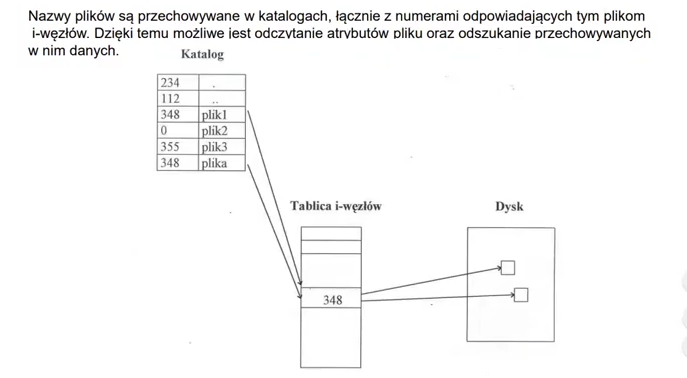
\includegraphics[width=1\linewidth]{./img/so1-05.png}
\end{figure}

\subsection{Zadania}

Atrybuty plików
Polecenie ll (alias polecenia ls –l) pokazuje miedzy innymi czas
ostatniej modyfikacji pliku. Polecenie to z opcją –u pokazuje czas
ostatniego dostępu do pliku, natomiast z opcją -c pokazuje czas
ostatniej zmiany informacji przechowywanych w i-węźle.

O godz. 19:00 poleceniem

\begin{verbatim}
$ /usr/bin/date > abc
\end{verbatim}
utworzono plik abc, po czym sprawdzono atrybuty tego pliku:

\begin{verbatim}
$ ll abc
-rw-r--r-- 1 user1 users 29 Sep 13 19:00 abc
\end{verbatim}

Następnie o godz. 19:10 wydano polecenie:

\begin{verbatim}
$ /usr/bin/date >> abc
\end{verbatim}

Podaj dokładnie co pokażą poniższe polecenia i uzasadnij odpowiedź:

\begin{verbatim}
$ ll abc
$ ll -u abc
$ ll -c abc
\end{verbatim}

O godz. 19:20 wydano polecenie:

\begin{verbatim}
$ ln abc xyz
\end{verbatim}
Podaj dokładnie co pokażą poniższe polecenia i uzasadnij odpowiedź:

\begin{verbatim}
$ ll abc
$ ll -u abc
$ ll -c abc
\end{verbatim}
O godz. 19:25 wydano polecenie:

\begin{verbatim}
$ chmod +x abc
\end{verbatim}
Podaj dokładnie co pokażą poniższe polecenia i uzasadnij odpowiedź:

\begin{verbatim}
$ ll xyz
$ ll -u xyz
$ ll -c xyz
\end{verbatim}

\subsection{Rozwiązanie}

Atrybuty plików
Polecenie ll (alias polecenia ls –l) pokazuje miedzy innymi czas
ostatniej modyfikacji pliku. Polecenie to z opcją –u pokazuje czas
ostatniego dostępu do pliku, natomiast z opcją -c pokazuje czas
ostatniej zmiany informacji przechowywanych w i-węźle.

O godz. 19:00 poleceniem
\begin{verbatim}
$ /usr/bin/date > abc
\end{verbatim}

utworzono plik abc, po czym sprawdzono atrybuty tego pliku:

\begin{verbatim}
$ ll abc
-rw-r--r-- 1 user1 users 29 Sep 13 19:00 abc
\end{verbatim}


Następnie o godz. 19:10 wydano polecenie:

\begin{verbatim}
$ /usr/bin/date >> abc
\end{verbatim}


Podaj dokładnie co pokażą poniższe polecenia i uzasadnij odpowiedź:
Zmieniła się wielkość pliku dwukrotnie, ponieważ dopisujemy do
pliku kolejną informację co powiększa Jego rozmiar, w każdym z
przypadków.


\begin{verbatim}
$ ll abc
-rw-r--r-- 1 user1 users 58 Sep 13 19:10 abc
\end{verbatim}


W tym przypadku czas się zmienia jako czas
modyfikacji.


\begin{verbatim}
$ ll -u abc
-rw-r--r-- 1 user1 users 58 Sep 13 19:00 abc
\end{verbatim}

Tutaj czas odczytu się nie zmienia, czyli to czas utworzenia.


\begin{verbatim}
$ ll -c abc
-rw-r--r-- 1 user1 users 58 Sep 13 19:10 abc
\end{verbatim}


Tutaj zmienia się czas, ponieważ przez modyfikację rozmiaru
zmienia się także informacja o i-węźle.


O godz. 19:20 wydano polecenie:

\begin{verbatim}
$ ln abc xyz
\end{verbatim}


Podaj dokładnie co pokażą poniższe polecenia i uzasadnij odpowiedź:

Zmienia się liczba dowiązań na 2 oraz godzina na i-węźle


\begin{verbatim}
$ ll abc
-rw-r--r-- 2 user1 users 58 Sep 13 19:10 abc
\end{verbatim}


Czas modyfikacji się nie zmienia.


\begin{verbatim}
$ ll -u abc
-rw-r--r-- 2 user1 users 58 Sep 13 19:00 abc
\end{verbatim}


Czas dostępu również się nie zmienia.

\begin{verbatim}
$ ll -c abc
-rw-r--r-- 2 user1 users 58 Sep 13 19:20 abc
\end{verbatim}


Czas na i-węźle się zmienia, ponieważ utworzono dowiązanie.


O godz. 19:25 wydano polecenie:


\begin{verbatim}
$ chmod +x abc
\end{verbatim}



Podaj dokładnie co pokażą poniższe polecenia i uzasadnij odpowiedź:
Zmieniają się uprawnienia dostępu, czyli plik staje się wykonywalny


\begin{verbatim}
$ ll xyz
Rwxr -xr – x 2 user1 users 58 Sep 13 19:10 xyz*
\end{verbatim}


Zmienia się nazwa pliku, czas modyfikacji pozostaje bez zmian

\begin{verbatim}
$ ll -u xyz
Rwxr -xr – x 2 user1 users 58 Sep 13 19:00 xyz*
\end{verbatim}


Zmienia się nazwa pliku, czas odczytu pozostaje bez zmian


\begin{verbatim}
$ ll -c xyz
Rwxr -xr – x 2 user1 users 58 Sep 13 19:25 xyz*
\end{verbatim}


Zmienia się nazwa pliku i czas na i-węźle, ponieważ zmieniliśmy uprawnienia do pliku.

\section{Sposób przechowywania plików na dysku}

Do przechowywania danych na dysku system UNIX używa bloków i fragmentów.
Fragment jest najmniejszą jednostką przestrzeni dyskowej zajmowanej przez plik.
Rozmiar bloku jest całkowitą wielokrotnością rozmiaru fragmentu (stosunek rozmiaru
bloku do rozmiaru fragmentu nie może jednak przekraczać 8):

np. rozmiar bloku wynosi 8 kB a rozmiar fragmentu 2kB.

\subsection{Reguły przydzielania bloków i fragmentów}

1. Jeśli rozmiar pliku jest mniejszy niż rozmiar fragmentu, plikowi temu przydzielany jest
pierwszy wolny fragment.

2. Jeśli rozmiar pliku jest większy niż rozmiar fragmentu, ale mniejszy niż rozmiar bloku,
plikowi temu przydzielane są kolejne fragmenty należące do tego samego bloku.

3. Jeśli rozmiar pliku Jest większy niż rozmiar bloku, to plikowi przydzielana jest
odpowiednia liczba bloków, niekoniecznie znajdujących się obok siebie, o łącznym
rozmiarze nie przekraczającym rozmiaru pliku.

Pozostała część pliku umieszczana jest zgodnie z regułami 1 oraz 2.

Do przechowywania informacji o stanie wolnych bloków i fragmentów można
wykorzystać mapę bitową, na przykład dla bloków 8 kB i fragmentów 2 kB :

\begin{verbatim}
1110    1110    0100    0011    0000    0001

blok 0  blok 1  blok 2  blok 3  blok 4  blok 5  ... -.
\end{verbatim}
0 - fragment wolny

1 - fragment zajęty


\textbf{Kolejność adresów w i-węźle jest zgodna z kolejnością informacji w pliku!}

W bloku którego adres jest jako pierwszy, będzie pierwsza, początkowa część informacji.

\subsection{Struktura systemu plików}

Blok identyfikacyjny Tablica i-węzłów  Bloki danych

Podział dysków na partycje
Dyski bywają dzielone na sekcje
fizyczne. Taki podział ma szereg wad.
Do najważniejszych należą:
\begin{itemize}
\item nieefektywne wykorzystanie miejsca na dysku,
\item rozmiar sekcji (a w wyniku rozmiar systemu plików nie większy niż rozmiar dysku),
\item nie można zmienić rozmiarów sekcji (systemu plików)
\end{itemize}

Niektóre implementacje systemu UNIX wykorzystują partycje logiczne LVM 

Każda partycja (sekcja) jest traktowana jako niezależny wirtualny dysk. Jest reprezentowana przez plik specjalny (urządzenia), podobnie jak każdy dysk

W partycjach tworzone są systemy plików. Można je również wykorzystać jako obszary
wymiany (swap).
Systemy plików utworzone w poszczególnych partycjach muszą być dowiązane do
głównego systemu plików:

\begin{verbatim}
mount plik_specjalny_reprezentujący_partycję katalog
\end{verbatim}

Operacja odwrotna:

\begin{verbatim}
umount plik_specjalny_reprezyntujący_partycję
umount katalog
\end{verbatim}

Mechanizm dysku z ruchomymi głowicami

Różne sposoby przydziału miejsca na dysku

\begin{itemize}
\item Przydział ciągły
\item Przydział listowy
\item Przydział indeksowy
\end{itemize}

Metody dostępu do informacji pliku
\begin{itemize}
\item Dostęp sekwencyjny
\item Dostęp bezpośredni (swobodny)
\end{itemize}

Ilustracja ciągłego przydziału
miejsca na dysku

Ilustracja listowego przydziału
miejsca na dysku

Tablica przydziału plików (File Allocation Table)

Ilustracja indeksowego przydziału miejsca na dysku



\section{Zarządzanie procesami}

\subsection{Pojęcie procesu}

\subsection{Tworzenie, usuwanie, zawieszanie i odwieszanie procesów.}

\subsection{Komunikacja między procesami.}

\subsection{Szeregowanie procesów.}

\section{Zarządzanie pamięcią}

\subsection{Pamięć główna}

\subsection{Pamięć pomocnicza na dysku (obszar wymiany „swap”)}

\subsection{Pojęcie pamięci wirtualnej}

\subsection{Procesy wymiany}

\subsection{Procesy stronicowania i segmentacji}

\section{Zarządzania operacjami wejścia wyjścia}

Podstawowe pojęcia (szyna, port we-wy, sterownik, odpytywanie, system przerwań)

Struktura oprogramowania we-wy w jądrze SO

Urządzenia znakowe, urządzenia blokowe

Pliki specjalne

Tablica rozdzielcza urządzeń

\section{Laboratorium}
\subsection{Podstawy użytkowania systemu}
Praca w systemie.

Postać poleceń w systemie UNIX .

\subsection{Wybrane polecenia podstawowe}

Polecenia służące identyfikacji użytkowników w systemie oraz komunikacji między użytkownikami.

\subsection{System plików}

Poruszanie się w systemie plików.

Tworzenie i usuwanie katalogów.

\subsection{Praca z plikami}

Plik i jego atrybuty .

Działania na plikach.

Dowiązywanie plików i katalogów.

\subsection{Prawa dostępu do plików i katalogów}
Podstawowe prawa dostępu

Zmiana praw dostępu.

\subsection{Podstawy edycji tekstów}
Edytory w systemie UNIX
Praca z edytorem vi
\subsection{Podstawy korzystania z shella}
Rodzaje shella

Wykonywanie poleceń w shellu

Środowisko shella
\subsection{Środowisko użytkownika}
Określanie środowiska użytkownika.
Zmienne shella
\subsection{Różne mechanizmy w shellu}
Generowanie nazw plików.
Przeadresowanie wejścia i wyjść
\subsection{Potoki}
Podstawianie poleceń
Korzystanie z wcześniej wydanych poleceń

\section{Wybrane polecenia działania na plikach tekstowych}
\subsection{Nadzorowanie wykonywania procesów}
Informacja o procesach
Przetwarzanie w pierwszym i drugim planie
Wysyłanie sygnałów do procesów
Planowanie wykonywania poleceń
\subsection{Wybrane polecenia użytkowe związane z archiwizacją plików}
Kompresja danych
Wyszukiwanie plików
Tworzenie kopii zapasowych
\subsection{Wprowadzenie do pracy w sieciach komputerowych}
Sieci komputerowe, sieć INTERNET
Poczta elektroniczna
Praca na zdalnym komputerze

\section{Literatura}

A. Silberschatz, P.B. Galvin, G. Gaigne; Podstawy systemów operacyjnych, WNT,
Warszawa 2005.

M. J. Bach; Budowa systemu operacyjnego UNIX, WNT, Warszawa, 1995.

B. Goodheart, J. Cox; Sekrety magicznego ogrodu, Unix system V wersja 4 od środka,
WNT, Warszawa, 2001.

B. Goodheart, J. Cox; Sekrety magicznego ogrodu, Unix system V wersja 4 od środka, - klucz do zadań. WNT, Warszawa, 2001.

K. Haviland, D. Gray, B. Salama; UNIX. Programowanie systemowe. Wydawnictwo RM,
Warszawa, 1999.

A. Silberschatz, P.B. Galvin, G. Gaign; Operating System Concepts. John Wley \& Sons, Inc., 2003.

A. S. Tanenbaum; Modern Operating Systems, Prentice-Hall, Inc. London, 1992.

E. Nemeth, G. Snyder, S. Seebass, T.R. Hein: Przewodnik administratora systemu UNIX. WNT, Warszawa, 1998.

S. Prata, D. Martin; Biblia systemu UNIX V. Polecenia i programy użytkowe, LT\&P, Warszawa, 1994.

A. Southerton, E.C. Perkins; Słownik poleceń systemów UNIX i X, Wiley \& WNT, Warszawa , 1995.

L. Lamb; Learning the vi editor. O'Reilly \& Associates, Inc., Sebastopol, CA, 1996.

M.I. Bolsky, D.G. Korn; The Kornshell - command and programming language, Prentice Hall,
1989.



\end{document}